\chapter{Architektur}
\label{cha:architektur}
In diesem Kapitel werden die architektonischen Randbedingungen für die Entwicklung der Applikation beschrieben. Hierzu zählt, welche Anwendungsfälle in die späteren Prototyp und im Messeprototyp gegeben sein sollen. Daraus resultiert der Aufbau der Datenbank und die schlussendliche Systemarchitektur. Als Grundlage dient das Pflichtenheft. Dieses liegt dieser Arbeit gesondert im Anhang bei (siehe Kapitel \ref{sec:Pflichtenheft}). Der Arbeitstitel dieses Projekts wird, in Anlehnung an ein Fitness-IT-Projekt, \textit{fIT} lauten. 

\section{Anwendungsfälle}
\label{sec:anwendungsfaelle}
Das Pflichtenheft sieht eine Unterteilung des Projekts in zwei aufeinanderfolgende Meilensteine vor (siehe Kapitel \ref{sec:meilenstein-plan}). Hierbei werden erst Proof-of-Concept-Prototyp entwickelt. Anschließend wird ein Prototyp zum Messeprototyp weiterentwickelt. \\
Für diese beiden Prototypen müssen andere bzw. erweiterte Anwendungsfälle implementiert werden. Aus diesem Grund werden nachfolgend für die beiden Implementierungsschritte die Anwendungsfälle einzeln aufgeschlüsselt. 
\subsection{Anwendungsfälle für Meilenstein 1 (Proof-of-Concept-Phase)}
\label{ssec:anwendungsfaelle-poc}
Aus dem Pflichtenheft ergeben sich folgende Anwendungsfälle für die erste Phase des Projekts (siehe Abbildung \ref{pic:usecase-poc}):
\begin{itemize}
\item Es soll möglich sein, sich an der Anwendung anzumelden.
\item Es soll möglich sein, eine Entität mit Daten (Trainingsplan, Training oder Übung), unabhängig von der Verbindung zum Web Service, persistent anzulegen, zu ändern und zu speichern.
\item Optional soll sich ein Nutzer an der Anwendung registrieren können.
\end{itemize}

\begin{figure}[h]
\centering
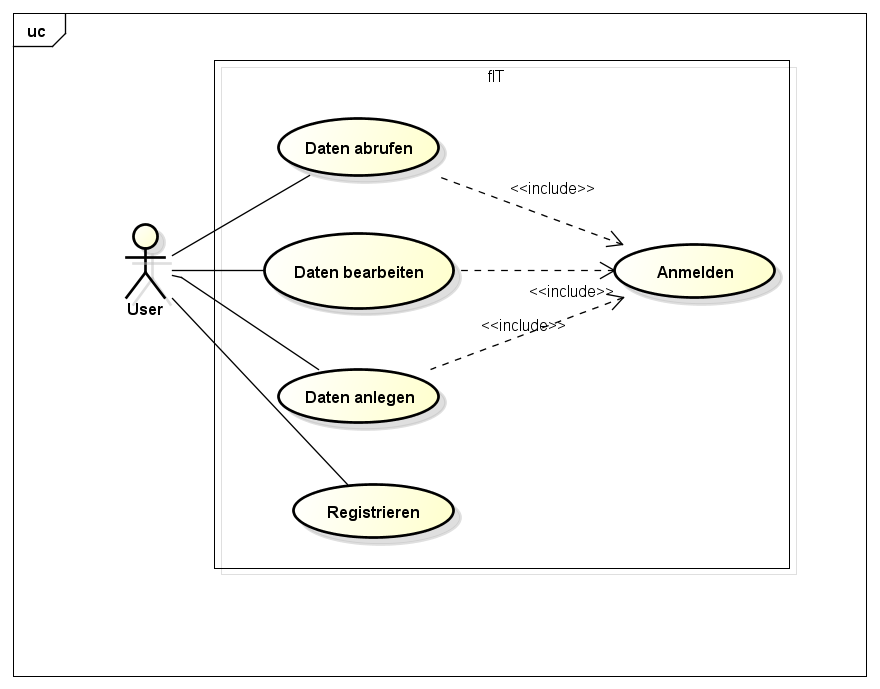
\includegraphics[width=0.8\linewidth]{content/images/UseCase-Proof-of-Concept.png}
\caption{Anwendungsfälle des \textit{Proof-of-Concept}-Prototyp}
\label{pic:usecase-poc}
\end{figure}

\subsection{Anwendungsfälle für Meilenstein 2 (Messeprototyp-Phase)}
\label{ssec:anwendungsfaelle-messe}
Für den Meilenstein 2 werden die bereits vorgestellten Anwendungsfälle weiter verfeinert. Daraus ergeben sich folgende Anwendungsfälle (siehe Abbildung \ref{pic:usecase-messe}):
\begin{itemize}
\item Ein Nutzer soll sich an der Anwendung anmelden können.
\item Ein Nutzer soll seine eigenen Trainingsplan-Daten abrufen können.
\item Ein Nutzer soll zu einem seiner Trainingspläne alle zugehörigen Übungen abrufen können.
\item Ein Nutzer soll zu einer dieser Übungen seine bisherigen Trainingsdaten abrufen können.
\item Ein Nutzer soll zu einer Übung ein neues Training anlegen können.
\item Alle nicht-optionalen Anwendungsfälle müssen unabhängig von einer Serververbindung funktionieren und eventuell anfallende Daten dauerhaft speichern.
\item Optional: Ein Nutzer soll eine Statistik der letzten Trainingsdaten zu einer Übung abrufen können. Neu erstellte Trainingsdaten aktualisieren diese Statistik.
\item Optional: Ein Nutzer soll sich an der Applikation registrieren können.
\item Optional: Ein Nutzer mit der Rolle \textit{Administrator} soll neue Übungen anlegen können.
\end{itemize}

\begin{figure}[h]
\centering
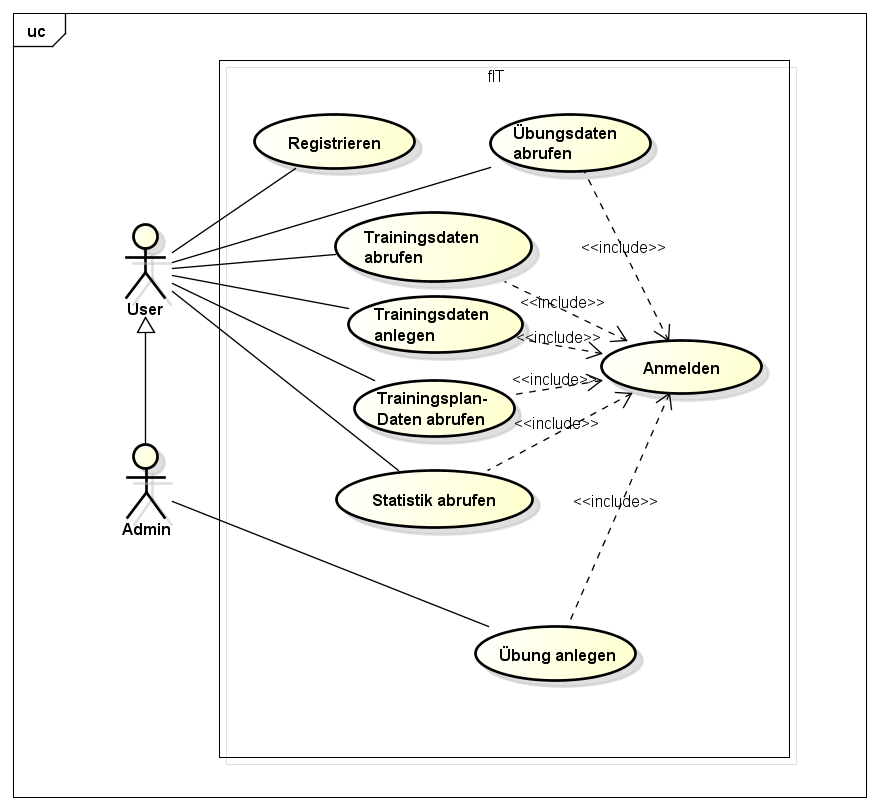
\includegraphics[width=0.8\linewidth]{content/images/UseCase-Messeprototyp.png}
\caption{Anwendungsfälle des Messeprototyp}
\label{pic:usecase-messe}
\end{figure}
\newpage
\section{Datenbank-Entwurf}
\label{sec:Datenbank-Entwurf}
Aus den definierten Anwendungsfällen ergibt sich die Struktur für die Datenbank. Diese wird in Abbildung \ref{pic:db-entwurf} dargestellt. Als Grundlage werden die Anwendungsfälle des zweiten Meilensteins genutzt, um spätere Anpassungen nach Beendigung des ersten Meilensteins zu vermeiden.

\begin{figure}[h]
\centering
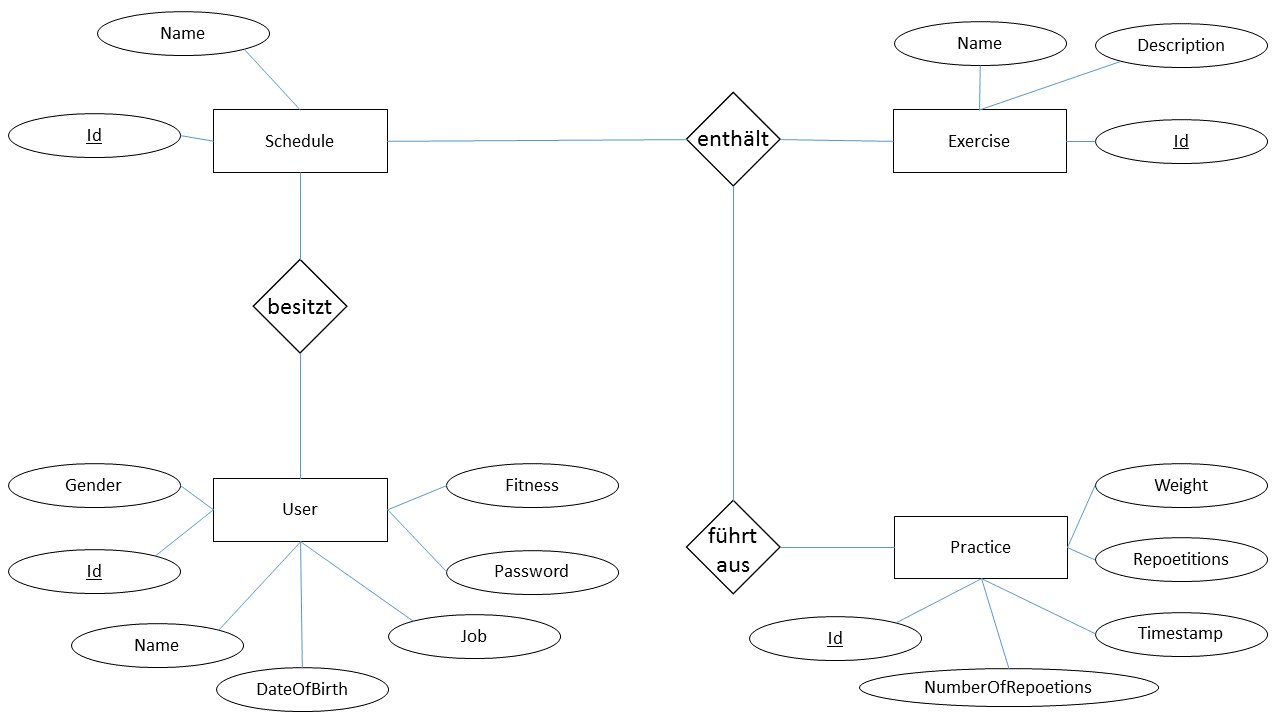
\includegraphics[width=0.8\linewidth]{content/images/DB-Entwurf.png}
\caption{Datenbank-Entwurf}
\label{pic:db-entwurf}
\end{figure}

\section{Programmarchitektur}
\label{sec:programmarchitektur}
Da verschiedene Clients implementiert werden sollen, ist es sinnvoll das Projekt als Mehrschichtenarchitektur für eine verteilte Anwendung zu implementieren. \\
Der Server stellt dabei die Funktionen zur Nutzung durch die Clients bereit. Konkret greift der Server per \gls{OR-Mapper} auf die Datenbank zu, bereitet die Daten in der Applikationsschicht auf und reicht sie über eine \ac{REST}-Schnittstelle an den anfragenden Client weiter. Eine detaillierte Beschreibung zu \ac{REST} wird in Kapitel \ref{sec:definition-rest} gegeben. Bei dieser Kommunikation muss gewährleistet sein, dass ein Nutzer nur die Daten abrufen darf, für die er autorisiert wurde. \\
Clientseitig werden Daten in einem lokalen Speicher zum Schutz vor eventuellen Verbindungsabbrüchen zwischengespeichert. Anschließend werden die erhaltenen Daten auf dem Endgerät für die Anzeige aufbereitet und angezeigt. \\
Abbildung \ref{pic:architecture} bildet diesen Aufbau grafisch ab:
\begin{figure}[h]
\centering
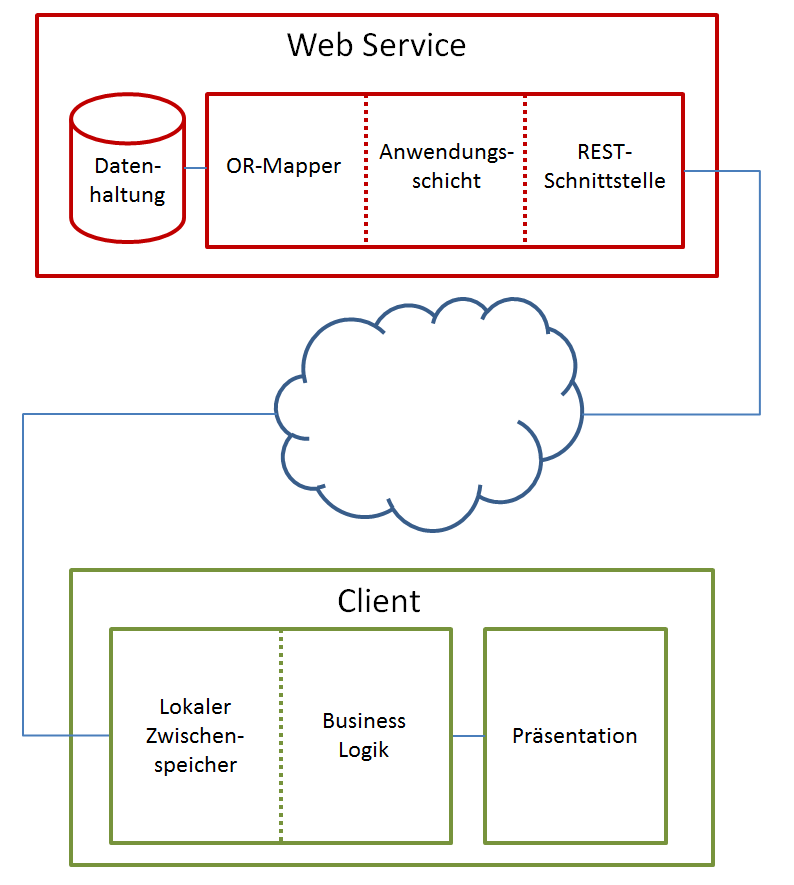
\includegraphics[width=0.7\linewidth]{content/images/Aufbau-Architektur.png}
\caption{Aufbau der Anwendung}
\label{pic:architecture}
\end{figure}

\newpage
\section{Rollen-Konzept}
\label{sec:rollen-konzept}
Im Pflichtenheft wird für den zweiten Meilenstein eine Unterscheidung im Bereich der Berechtigungen vorgenommen. So dürfen beispielsweise nur Administrationen neue Übungen anlegen. Aus diesem Grund ist es notwendig, ein Rollenkonzept zu entwickeln, welches den Zugriff auf bestimmte Ressourcen reguliert. \\
Aus den Aussagen, die im Pflichtenheft getroffen wurden, geht hervor, dass sich der Nutzer in einer der nachfolgenden Status befindet, wenn er auf den Web Service zugreifen will: 
\begin{itemize}
\item unautorisiert \\
Der Nutzer hat sich noch nicht gegenüber des Web Servers authentifiziert. In diesem Status kann der Nutzer sich mit seinen Anmeldedaten einloggen oder als neuer Nutzer an der Web \ac{API} registrieren.
\item Rolle \textbf{Nutzer}\\
Jeder angemeldete Nutzer besitzt die Rolle \textit{Nutzer}. Ein normaler Nutzer kann seine Daten einsehen. Dies beinhaltet seine Trainingspläne, deren Übungen und die dazu angelegten Trainingseinheiten.
\item Rolle \textbf{Administrator}\\
Ein \textit{Administrator} ist ebenfalls ein Nutzer. Er kann zusätzlich neue Übungen anlegen. 
\end{itemize}